% Snowflake Data Engineering — Chapter 13 | original manuscript draft
% Author: Arman Golbidi | Editorial snapshot: 22 October 2026
% Compile: xelatex -interaction=nonstopmode -halt-on-error Snowflake_Data_Engineering_Chapter_13.tex
% Trim: 178 x 254 mm; margins inside 23 mm / outside 17 mm / top-bottom 19 mm.
% Body: 10.75 pt / 13.65 pt leading = 1.27 line-height ratio; code: 8.75 pt.
\documentclass[11pt,twoside]{article}
\usepackage[paperwidth=178mm,paperheight=254mm,inner=23mm,outer=17mm,top=19mm,bottom=19mm,headheight=5mm,headsep=4mm,footskip=9mm]{geometry}
\usepackage{fontspec}
\setmainfont{LibertinusSerif-Regular.otf}[BoldFont=LibertinusSerif-Bold.otf,ItalicFont=LibertinusSerif-Italic.otf,BoldItalicFont=LibertinusSerif-BoldItalic.otf]
\setsansfont{LibertinusSans-Regular.otf}[BoldFont=LibertinusSans-Bold.otf,ItalicFont=LibertinusSans-Italic.otf]
\setmonofont{LibertinusMono-Regular.otf}[Scale=0.91]
\usepackage[english]{babel}
\usepackage{microtype}
\usepackage{setspace}
\setstretch{1.0}
\usepackage{titlesec,enumitem,tabularx,array,booktabs,needspace,fancyhdr,lastpage}
\usepackage[most]{tcolorbox}
\usepackage{tikz}
\usetikzlibrary{arrows.meta,positioning,fit,shapes.misc,calc}
\usepackage{listings}
\usepackage{xcolor}
\usepackage{hyperref}
\usepackage{amsmath}
\hypersetup{colorlinks=true,urlcolor=steelblue,linkcolor=steelblue,pdfauthor={Arman Golbidi},pdftitle={Snowflake Data Engineering - Chapter 13: Security, Governance, Reliability, and Cost},pdfsubject={English technical book manuscript, thirteenth chapter, 178 x 254 mm}}
\definecolor{navy}{HTML}{15334A}
\definecolor{steelblue}{HTML}{17779B}
\definecolor{teal}{HTML}{12888A}
\definecolor{lightblue}{HTML}{ECF5F7}
\definecolor{papergray}{HTML}{F2F5F6}
\definecolor{inkgray}{HTML}{4A5862}
\definecolor{thinrule}{HTML}{CBD7DB}
\AtBeginDocument{\color{navy}\fontsize{10.75}{13.65}\selectfont}
\setlength{\parindent}{0pt}
\emergencystretch=2.5em
\setlength{\parskip}{3.3pt plus 0.7pt minus 0.6pt}
\setlist[itemize]{leftmargin=4mm,itemsep=1pt,topsep=2pt,parsep=0pt}
\setlist[enumerate]{leftmargin=5mm,itemsep=1pt,topsep=2pt}
\titleformat{\section}{\sffamily\bfseries\color{navy}\fontsize{14}{17}\selectfont}{}{0pt}{}
\titlespacing*{\section}{0pt}{8pt}{4pt}
\titleformat{\subsection}{\sffamily\bfseries\color{steelblue}\fontsize{10.8}{13}\selectfont}{}{0pt}{}
\titlespacing*{\subsection}{0pt}{5pt}{1pt}
\newcommand{\topic}[2]{\subsection*{#1\quad #2}}
\newcommand{\repo}[2]{\par\begingroup\fontsize{8.0}{9.6}\selectfont\sffamily\color{inkgray}\textbf{Project reference:} \href{#2}{#1}. \textit{Not independently executed; rights review pending.}\par\endgroup}
\newtcolorbox{insight}[1][]{enhanced,breakable,colback=lightblue,colframe=thinrule,boxrule=.45pt,arc=1.3mm,left=2.8mm,right=2.8mm,top=1.8mm,bottom=1.8mm,before skip=5pt,after skip=5pt,#1}
\newtcolorbox{whitebox}[1][]{enhanced,breakable,colback=papergray,colframe=thinrule,boxrule=.35pt,arc=1mm,left=2.6mm,right=2.6mm,top=1.5mm,bottom=1.5mm,before skip=4pt,after skip=5pt,#1}
\lstdefinestyle{chaptercode}{basicstyle=\ttfamily\fontsize{8.75}{10.7}\selectfont,backgroundcolor=\color{papergray},frame=single,framerule=.35pt,rulecolor=\color{thinrule},breaklines=true,columns=fullflexible,keepspaces=true,showstringspaces=false,aboveskip=5pt,belowskip=5pt,xleftmargin=2mm,xrightmargin=1mm,framexleftmargin=2mm,framexrightmargin=1mm}
\lstset{style=chaptercode}
\pagestyle{fancy}
\fancyhf{}
\fancyhead[LE]{\sffamily\fontsize{7.6}{9}\selectfont\color{inkgray}\textsc{Snowflake Data Engineering}}
\fancyhead[RO]{\sffamily\fontsize{7.6}{9}\selectfont\color{inkgray}\textsc{13 / Governance \& Cost}}
\fancyfoot[LE,RO]{\sffamily\bfseries\fontsize{8.2}{9}\selectfont\color{steelblue}\thepage}
\fancyfoot[LO,RE]{\sffamily\fontsize{7.6}{9}\selectfont\color{inkgray}Arman Golbidi \quad | \quad Chapter 13}
\renewcommand{\headrulewidth}{0.35pt}
\renewcommand{\footrulewidth}{0pt}
\setcounter{page}{227}
\raggedbottom

\begin{document}
% PAGE 227
{\sffamily\bfseries\fontsize{9}{11}\selectfont\color{steelblue} CHAPTER 13 \hfill TRUST / RECOVERY / UNIT ECONOMICS}\par\vspace{3mm}
{\sffamily\bfseries\fontsize{20}{23}\selectfont\color{navy} Security, Governance,\\Reliability, and Cost}\par\vspace{2mm}
{\sffamily\fontsize{11}{14}\selectfont\color{steelblue} When a data platform works technically, who ensures it is safe to trust?}\par\vspace{3mm}
\begin{insight}\textbf{The dashboard was correct, but the delivery was not.}\par
A Finnish energy analyst opens a carefully reconciled generation dashboard: six accepted observations, 66.000 MWh in the synthetic teaching fixture. An hourly service identity powers the refresh. It also happens to have the power to delete the raw feed, read an unrelated customer directory, and create an unrestricted warehouse. Nobody noticed until a mistaken deployment revoked the report's access and an unattended workload kept running after the analyst went home. Correct numbers alone did not make this a reliable data product.
\end{insight}
The architecture built through Chapters~3--12 now has a second contract: protect what the product knows, account for what it spends, and recover from what will go wrong. Security is an engineering property of roles, boundaries and tested denial. Governance identifies who owns meaning and decisions. Reliability translates incidents into rehearsed action. Cost management gives those decisions a financial constraint. None can be outsourced to a single configuration switch.
\begin{whitebox}\textbf{Learning outcomes}\par
After this chapter, you can (1) draw a threat boundary and least-privilege role graph; (2) distinguish masking and row-access policies from access grants; (3) design identity, tagging, auditing and privacy controls; (4) attribute warehouse and serverless usage without inventing prices; (5) explain the different coverage of monitors and budgets; (6) develop an incident runbook with measurable recovery objectives; and (7) execute negative-access and cost-ledger checks in a safe lab.
\end{whitebox}
\textbf{Prerequisites.} Chapters~3, 5, 10 and 12, and a basic understanding of schemas, roles and query history. Exercises are designed around \emph{synthetic} energy data. Live Snowflake security policies may require Enterprise Edition, administrator approval, and billable resources; do not deploy these examples to shared or production environments without review.
\begin{center}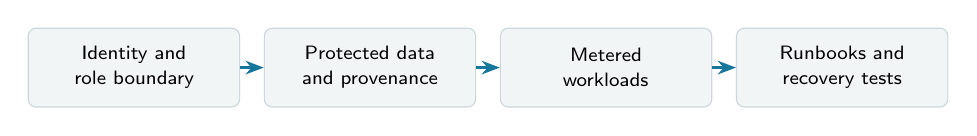
\begin{tikzpicture}[>=Stealth,every node/.style={font=\sffamily\fontsize{7.5}{9}\selectfont},n/.style={draw=thinrule,rounded corners=1mm,fill=papergray,align=center,text width=24.5mm,minimum height=10mm}]
\node[n](a){Identity and\\role boundary};\node[n,right=3mm of a](b){Protected data\\and provenance};\node[n,right=3mm of b](c){Metered\\workloads};\node[n,right=3mm of c](d){Runbooks and\\recovery tests};
\draw[->,thick,steelblue](a)--(b);\draw[->,thick,steelblue](b)--(c);\draw[->,thick,steelblue](c)--(d);
\end{tikzpicture}\\{\fontsize{8}{9}\selectfont\color{inkgray}Figure 13.1. Trust requires identity, data, expense and recovery controls together.}\end{center}
\newpage
% PAGE 228
\section*{13.1\quad Security architecture and least privilege}
\topic{13.1.1}{Threat boundaries and trust assumptions}
Consider five actors around the energy platform: an ingestion service, a transformation runner, a dashboard reader, a platform operator and an external data recipient. Their credentials, networks, data domains and actions differ. Draw boundaries between the identity provider, client device, Snowflake account, storage or external integrations, reporting workspace and downstream consumers. At every boundary ask: \emph{Who can impersonate whom, see which records, trigger what execution, or obtain a secret?}

A threat model is not an assertion that the cloud platform is insecure. It makes assumptions explicit. In our exercise we assume the identity provider controls human SSO; privileged Snowflake administration is separated from routine querying; source files are untrusted until validated; and application operators cannot silently change security policy. Identify adverse events: exposed PAT or private key, broad grant to a role, malicious SQL in an unsafe client, incorrect masking context, unrestricted outgoing integration, and accidental sharing of a raw table.
\begin{whitebox}\textbf{Threat boundary worksheet}\par
\textbf{Asset:} energy readings and contact metadata. \textbf{Actor:} scheduled loader. \textbf{Permitted:} insert into a designated landing table and use a small warehouse. \textbf{Forbidden:} create users, read contact details, grant roles and export to an unrelated destination. \textbf{Control:} scoped role plus protected secret. \textbf{Evidence:} denied operations, access events and grant-diff review.
\end{whitebox}
\topic{13.1.2}{Privilege minimization begins at the task}
Start from a job statement and derive precisely the privileges it requires. A Power BI consumer normally needs usage on its warehouse and parent containers plus select on approved serving objects, not ownership of source tables. An ingest worker may need insert or a scoped load operation, not unrestricted access to every schema. Privilege reduction is also temporal: a migration or incident role can be activated for an approved window rather than granted permanently.

\textbf{Common failure.} A service identity has \texttt{ACCOUNTADMIN} because setup was easier. This combines credentials, powerful access and continuous machine execution into a large blast radius. Replace it with purpose-built account or database roles, limit secrets to the runtime that needs them, and require an independently reviewed escalation path.
\repo{P142: Snowflake Horizon governance guide}{https://github.com/Snowflake-Labs/sfguide-getting-started-with-horizon-data-governance-in-snowflake}
\textbf{Check.} Can each permission in the architecture be traced to a business operation and an owner?
\newpage
% PAGE 229
\topic{13.1.3}{Separation of duties and audits}
Separation of duties breaks the chain from authoring a change to silently authorizing, deploying and hiding it. A data engineer can propose a new masked field; a governance steward approves the classification; a security operator approves the grant and policy; a release pipeline deploys an auditable artifact. Small teams may combine roles, but should still require a separate reviewer for high-impact changes and retain the decision record. The key distinction is between accountability and technical privilege: a person might own an outcome without holding unrestricted database rights.
\begin{center}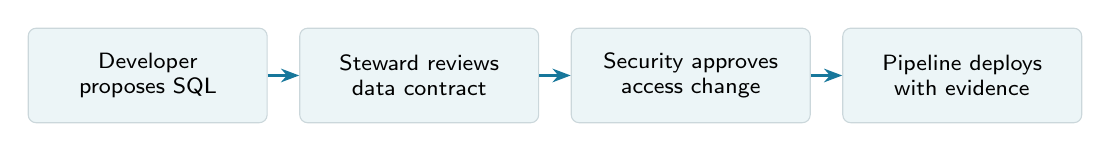
\begin{tikzpicture}[>=Stealth,every node/.style={font=\sffamily\fontsize{8}{9}\selectfont},n/.style={draw=thinrule,rounded corners=1mm,fill=lightblue,align=center,text width=28mm,minimum height=12mm}]
\node[n](a){Developer\\proposes SQL};\node[n,right=4mm of a](b){Steward reviews\\data contract};\node[n,right=4mm of b](c){Security approves\\access change};\node[n,right=4mm of c](d){Pipeline deploys\\with evidence};
\draw[->,steelblue,thick](a)--(b);\draw[->,steelblue,thick](b)--(c);\draw[->,steelblue,thick](c)--(d);
\end{tikzpicture}\\{\fontsize{8}{9}\selectfont\color{inkgray}Figure 13.2. A reviewed change creates evidence before it reaches consumers.}\end{center}
A good audit record has the change ID, requester, approver, affected account and objects, before/after grants, linked SQL commit, test evidence, deployment identity and rollback plan. Logs cannot substitute for prevention: detecting a data export after the data has left is too late. Conversely, access restriction without evidence can conceal a broken data product for days. Put both in the control design.
\begin{lstlisting}[language=SQL,caption={Read-only inspection; use a dedicated approved review role.}]
SHOW GRANTS TO ROLE BOOK13_READER;
SHOW GRANTS ON TABLE BOOK13_SANDBOX.RAW.METER_EVENT;
-- Change documentation is external to these results:
-- approval ID; captured timestamp; release commit.
\end{lstlisting}
The current role and any active secondary roles affect authorization; policy tests must record session context. A successful \texttt{SELECT} by an administrator does not show that a reader role is safe. A denied \texttt{SELECT} from a restricted role is valuable evidence, provided the test actually ran under that role rather than inheriting broader permissions.
\begin{insight}\textbf{Decision rule.} For every control ask both questions: ``What will this prevent?'' and ``How will we detect a regression?'' A defensible answer names a scoped object, an owner, an automated check and a human review cadence.\end{insight}
\newpage
% PAGE 230
\subsection*{Audit closure: evidence, not screenshots alone}
Treat an approval, a negative-access query, and a query-history record as three different kinds of evidence. Approval proves authorization to change; an access test proves an expected behavior under a stated session; a history record helps reconstruct what was run. None independently proves continuing compliance. Repeat policy assertions after role migrations, identity provider changes and upgrades to reporting integrations.

Choose tests that fail when someone broadens access accidentally. For example, a dashboard-reader role must not be able to select \texttt{RAW.METER\_EVENT}, insert into \texttt{GOLD.GENERATION\_DAILY} or assume the ingestion role. Verify the corresponding positive behavior as well: that the reader \emph{can} query an approved, masked serving view. A permission system that denies everything is not a functioning product.
\begin{whitebox}\textbf{Regression case: new inherited privilege}\par
A reviewer grants \texttt{BOOK13\_READER} a parent role to simplify deployments. The new hierarchy unexpectedly inherits \texttt{SELECT} on raw contact records. A grant-diff check flags the unexpected edge, while an authorized-session probe demonstrates the new access. Roll back the role edge, not just the user assignment, and rerun the negative-access suite.
\end{whitebox}
\textbf{What to capture:} timestamp, role graph snapshot, policy DDL, object inventory, permitted and denied query IDs, incident ticket, evaluator and limitations. An offline model of the role graph is useful for reasoning but does not replace an actual Snowflake permission test. Where audit views have latency or require a licensed feature, state that limitation rather than treating missing rows as evidence of safety.

\textbf{Trade-off.} More tightly scoped roles increase administration overhead; broad roles lower initial friction but enlarge impact and undermine explainability. Prefer reusable access roles combined into functional roles and automate their review. Chapter~10's release checklist should require a security diff just as it requires data-quality and schema compatibility tests.
\textbf{Check.} Could a teammate reproduce an access-denied assertion from an archived release record, without borrowing an administrator session?
\newpage
% PAGE 231
\section*{13.2\quad Role-based access control and role hierarchies}
\topic{13.2.1}{Role hierarchy design}
Snowflake uses grants to roles and role inheritance. Model the \emph{minimum} object privileges first, then compose them into functional roles. For the energy case, \texttt{BOOK13\_RAW\_WRITER} writes an isolated raw table, \texttt{BOOK13\_GOLD\_READER} reads serving tables, and \texttt{BOOK13\_ANALYST} inherits only the latter. Database roles can scope object grants inside a database; account roles hold warehouse privileges and are active in sessions. Account roles may inherit database roles, but database roles cannot inherit account roles.
\begin{center}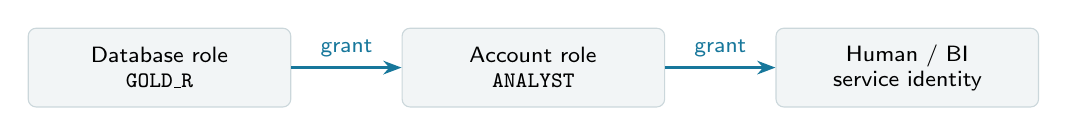
\begin{tikzpicture}[>=Stealth,every node/.style={font=\sffamily\fontsize{7.6}{9}\selectfont},n/.style={draw=thinrule,rounded corners=1mm,fill=papergray,align=center,text width=31mm,minimum height=10mm}]
\node[n](low){Database role\\\texttt{GOLD\_R}};\node[n,right=14mm of low](func){Account role\\\texttt{ANALYST}};\node[n,right=14mm of func](user){Human / BI\\service identity};
\draw[->,steelblue,thick](low)--node[above]{grant}(func);\draw[->,steelblue,thick](func)--node[above]{grant}(user);
\end{tikzpicture}\\{\fontsize{8}{9}\selectfont\color{inkgray}Figure 13.3. Grant direction matters: parent roles inherit child privileges.}\end{center}
\topic{13.2.2}{Object ownership and grants}
\texttt{OWNERSHIP} is powerful: it controls an object and influences who can grant access. In a managed access schema, grants on contained objects are centrally managed by the schema owner or a role with \texttt{MANAGE GRANTS}; object owners do not grant access themselves. Choose managed access for governed serving zones when centralized approval matters, but document the resulting administration requirements. Avoid automatic future grants until the whole object class has a consistent sensitivity profile.
\begin{lstlisting}[language=SQL,caption={Illustrative administrator-approved setup, isolated sandbox.}]
CREATE ROLE IF NOT EXISTS BOOK13_ANALYST;
GRANT USAGE ON DATABASE BOOK13_SANDBOX
  TO ROLE BOOK13_ANALYST;
GRANT USAGE ON SCHEMA BOOK13_SANDBOX.GOLD
  TO ROLE BOOK13_ANALYST;
GRANT SELECT ON TABLE
  BOOK13_SANDBOX.GOLD.GENERATION_DAILY
  TO ROLE BOOK13_ANALYST;
-- Warehouse USAGE is granted separately.
\end{lstlisting}
\repo{P024: Terraform Snowflake RBAC example}{https://github.com/Infostrux-Solutions/terraform-snowflake-rbac-infra}
\newpage
% PAGE 232
\topic{13.2.3}{Permission regression tests}
Your access model is a graph, not a spreadsheet of names. Suppose \texttt{BOOK13\_ANALYST} is later granted \texttt{BOOK13\_LOADER}; its new effective privileges may exceed the design even if no direct raw-table grant was added. Review role-to-role edges, role-to-user assignments, database roles and active secondary roles. Testing only direct grants misses inherited privilege.

\begin{whitebox}\textbf{Acceptance matrix for the sandbox}\par
\begin{tabularx}{\linewidth}{>{\raggedright\arraybackslash}Xcc}
\toprule
Operation & Analyst & Loader \\
\midrule
Read \texttt{GOLD.GENERATION\_DAILY} & Allow & Deny \\
Read \texttt{RAW.METER\_EVENT} & Deny & As scoped \\
Insert into raw event table & Deny & Allow \\
Create account user or grant roles & Deny & Deny \\
\bottomrule
\end{tabularx}
\end{whitebox}
Use actual dedicated test identities after an administrator approves the test. \texttt{USE ROLE} alone is insufficient if secondary roles remain active, the identity can assume additional roles, or a direct user grant is in effect. Set secondary-role behavior explicitly where permitted and record the active context. Never present a failed syntax statement as an access-control success: the negative test must fail for the expected authorization reason.
\begin{lstlisting}[language=SQL,caption={Reader probe: run only with the approved reader identity.}]
SELECT CURRENT_ROLE(), CURRENT_USER();
SELECT COUNT(*)
FROM BOOK13_SANDBOX.GOLD.GENERATION_DAILY;
-- Expected permission denial (separate statement):
SELECT COUNT(*)
FROM BOOK13_SANDBOX.RAW.METER_EVENT;
\end{lstlisting}
Tests also need boundaries: an authorized administrator can read or change many objects; a test runner that assumes that role invalidates the evidence. An automated role-lint script can detect unwanted \texttt{GRANT} edges offline and should complement, never replace, real negative-access tests.
\repo{P143: Terraform role module}{https://github.com/getindata/terraform-snowflake-role}
\textbf{Check.} Which privilege, inherited by which path, could explain a newly successful query against the raw table?
\newpage
% PAGE 233
\section*{13.3\quad Authentication, secrets, and network controls}
\topic{13.3.1}{SSO and key-based authentication options}
Human access should normally be tied to an organization-managed identity, with appropriate single sign-on and multifactor controls. Programmatic clients may use a supported noninteractive authentication method such as key-pair authentication or an approved token-based integration. Authentication proves an identity; authorization still determines its roles and object privileges. Neither a private network nor SSO makes an overprivileged service account harmless.
\topic{13.3.2}{Secret rotation and vaulting}
Do not put passwords, connection strings or private keys in a Git repository, LaTeX example, dashboard parameter export or CI log. Store secrets in an approved vault or workload identity flow; restrict who can retrieve them and rotate on a planned schedule or immediately after suspected exposure. Record key owners, expiry alerts, rotation steps and safe decommissioning. A second valid credential permits a controlled transition without simultaneously breaking every refresh job.
\topic{13.3.3}{Network and endpoint controls}
Snowflake network rules and policies can restrict allowed or blocked network origins; authentication policies constrain allowed authentication methods. Roll out network changes in stages, retain an approved break-glass path and test from the actual connector location. A rule suitable for an office IP may block a cloud-hosted Power BI refresh service. Restrict outbound destinations through separate integration controls rather than assuming inbound network policy covers egress.
\begin{whitebox}\textbf{Operational check}\par
Before changing a network or authentication policy, identify supported client versions, remote worker locations, automation endpoints and fallback administrators. Require a successful human login and scheduled-job smoke test from authorized locations, with an agreed rollback window.
\end{whitebox}
\repo{P146: Securing a Snowflake account}{https://github.com/sfc-gh-jbellegarde/securing-your-snowflake-account}
\textbf{Check.} What would remain exposed if a service key were stolen but an IP allowlist were perfectly enforced?
\newpage
% PAGE 234
\section*{13.4\quad Masking policies, row access, and classification}
\topic{13.4.1}{Dynamic data masking}
Column masking changes what a permitted query returns based on policy logic and session context; it does not by itself grant table access. A masked contact identifier may remain hidden for analysts and visible to a designated steward. In Snowflake, dynamic data masking requires a supported edition (Enterprise Edition or higher as documented at this editorial checkpoint). Create and apply policies only in a permitted sandbox.
\begin{lstlisting}[language=SQL,caption={Illustrative masking policy; requires approved security role.}]
CREATE MASKING POLICY BOOK13_SANDBOX.GOV.EMAIL_MASK
  AS (val STRING) RETURNS STRING ->
  CASE WHEN IS_ROLE_IN_SESSION('BOOK13_STEWARD')
       THEN val ELSE '[MASKED]' END;
-- Attach in the approved security deployment:
ALTER TABLE BOOK13_SANDBOX.GOLD.CONTACT_CONTEXT
  MODIFY COLUMN CONTACT_EMAIL SET MASKING POLICY
  BOOK13_SANDBOX.GOV.EMAIL_MASK;
\end{lstlisting}
\topic{13.4.2}{Row access policies}
Row access policies decide which records a role can see, for example only an authorized plant region. They are evaluated at query time and do not automatically stop unauthorized inserts. Use ordinary grants to stop writes and row policies to constrain qualifying reads. Avoid a policy that relies on caller-controlled session variables for sensitive authorization without a protected mapping.
\topic{13.4.3}{Classification and authorized test users}
Classify by sensitivity and business need: public aggregate, internal operational, confidential contact metadata and regulated personal data. Validate masking for a real approved reader and a real steward. Verify both positive and negative cases and protect the evidence itself: a screenshot of unmasked sensitive values can be a new exposure.
\repo{P147: Snowflake security demonstration}{https://github.com/aballingall/snowflake-security-demo}
\textbf{Check.} Why can a policy return masked values to a reader even after \texttt{SELECT} has been granted?
\newpage
% PAGE 235
\section*{13.5\quad Tags, lineage, auditing, and data sharing}
\topic{13.5.1}{Tags and lineage provenance}
A governance tag supplies machine-readable metadata such as \texttt{DATA\_CLASS = INTERNAL} or \texttt{COST\_CENTER = ENERGY}. It is useful for discovery and reporting, but a label does not enforce access unless linked to a specific policy and verified. Store a data dictionary that connects each column's meaning to its source, refresh logic, owner and retention decision. Separate structural lineage (object A depends on B) from event-level lineage (this accepted row was derived from source file X under transform release Y).
\begin{center}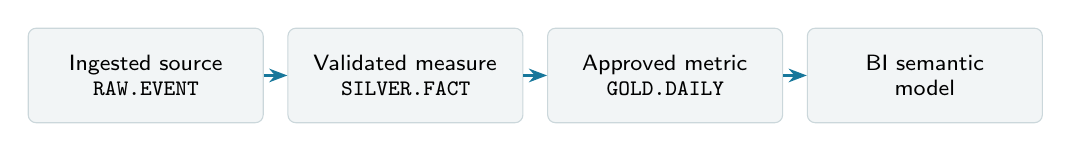
\begin{tikzpicture}[>=Stealth,every node/.style={font=\sffamily\fontsize{7.6}{9}\selectfont},n/.style={draw=thinrule,rounded corners=1mm,fill=papergray,align=center,text width=27.5mm,minimum height=12mm}]
\node[n](raw){Ingested source\\\texttt{RAW.EVENT}};\node[n,right=3mm of raw](silver){Validated measure\\\texttt{SILVER.FACT}};\node[n,right=3mm of silver](gold){Approved metric\\\texttt{GOLD.DAILY}};\node[n,right=3mm of gold](bi){BI semantic\\model};
\draw[->,steelblue,thick](raw)--(silver);\draw[->,steelblue,thick](silver)--(gold);\draw[->,steelblue,thick](gold)--(bi);
\end{tikzpicture}\\{\fontsize{8}{9}\selectfont\color{inkgray}Figure 13.4. Governance metadata must follow the whole measurement path.}\end{center}
\begin{lstlisting}[language=SQL,caption={Metadata inventory to support a governed review.}]
SHOW TAGS IN SCHEMA BOOK13_SANDBOX.GOV;
SELECT CURRENT_DATABASE(), CURRENT_SCHEMA();
-- Review lineage and catalog with an approved role;
-- exact availability and privileges are account-specific.
\end{lstlisting}
\textbf{Trade-off.} Attaching many tags without defined owners produces metadata noise. Start with a few required classifications tied to visible decisions, then verify completeness in release checks. Energy totals must retain provenance and units even when no personal information is involved.
\repo{P133: Intra-organization sharing guide}{https://github.com/Snowflake-Labs/sfguide-horizon-intra-organization-sharing}
\textbf{Check.} Can an analyst trace the value 66.000 MWh through the source version, accepted rows, model version and aggregation grain?
\newpage
% PAGE 236
\topic{13.5.2}{Access audit and usage history}
Security operations need to answer three questions: who ran a statement, which object was accessed and which policy or grant change enabled the behavior. Query History, Access History, Login History and Grant views serve related but different purposes; they have separate availability, privilege requirements and ingestion delays. A query record may show submitted text and execution time, while access history may enumerate objects accessed. Do not infer ``no access'' from an empty view before considering lag, retention, unsupported object types or insufficient viewing privileges.
\begin{lstlisting}[language=SQL,caption={Read-only audit pattern; account-usage rights required.}]
SELECT query_id, query_type, user_name,
       role_name, start_time
FROM SNOWFLAKE.ACCOUNT_USAGE.QUERY_HISTORY
WHERE start_time >= DATEADD(day, -1, CURRENT_TIMESTAMP())
  AND query_tag LIKE 'book13_%'
ORDER BY start_time DESC;
\end{lstlisting}
Protect audit records from broad access; query text can itself contain sensitive literals or identifiers. Keep operations evidence longer than a single incident when justified, but avoid collecting unbounded identity data. Prefer parameters instead of embedding secrets in SQL text. Define a minimal investigation record: time window, identity, role, object, query ID, user impact, hypothesis, evidence and response decision.
\begin{whitebox}\textbf{Investigation example}\par
A user reports seeing a column unexpectedly. First reproduce using the approved role and masked query. Then inspect relevant masking policy DDL and active role hierarchy; correlate query ID and deployment record. Only then decide whether the incident was a policy bug, a broadened grant, a changed semantic model or a misunderstanding of the reported value.
\end{whitebox}
\textbf{Check.} Which timestamps, log delays and privilege requirements would you document before claiming an access event is absent?
\newpage
% PAGE 237
\topic{13.5.3}{Secure sharing and policy enforcement}
Snowflake Secure Data Sharing can expose selected governed objects without creating a separate file-export pipeline. That is useful for partners, but the design question remains what the consumer may learn, not simply whether a share can be created. Prefer approved, stable projections over raw internal tables, document downstream interpretations and confirm row/column policies behave as expected in the intended sharing context. Some security features impose restrictions on shared objects; validate the complete combination before committing to a delivery promise.

A provider's share inventory should record: provider account and region, recipient account, dataset owner, field classifications, allowed purpose, change notice, expiration or revocation plan, applicable contractual review, and monitored usage. Do not assume that revoking future access deletes material a recipient has already copied or derived. Sharing and deletion are two different operational controls.
\begin{whitebox}\textbf{Data-product contract for a hypothetical regional partner}\par
Dataset: hourly wind generation aggregate. Allowed values: timestamp UTC, production region, MWh total, refresh timestamp. Excluded: personal contacts, source-system credentials, raw device identifiers. Service expectation: revised records within the agreed reporting window. Consumer test: known fixture reproduces the published totals and exposes no restricted columns. Revocation test: removal of the documented grant blocks further approved-account reads.
\end{whitebox}
Keep provenance visible after publication. The consumer needs to know whether a revised total replaces a previous total, whether a zero means observed zero or missing input, and whether daylight-saving conversions were applied. A secure share of semantically ambiguous data is still an unsafe data product.

\textbf{Incident case.} A BI refresh includes \texttt{SOURCE\_CONTACT\_EMAIL} after a schema evolution. The correct response is not merely to rename the column in Power BI. Contain the feed, remove the field from the shared projection, investigate who received the earlier output, test the new schema and document notification decisions with the appropriate owner and counsel.
\repo{P064: ShareWatch schema-drift monitor}{https://github.com/Snowflake-Labs/sfguide-monitor-schema-drift-in-data-shares-with-sharewatch}
\textbf{Check.} What can the provider technically revoke, and what cannot be guaranteed after a consumer has exported the result?
\newpage
% PAGE 238
\section*{13.6\quad Privacy, retention, and compliance basics}
\topic{13.6.1}{Personal data handling}
The running energy fixture is entirely synthetic. A real industrial platform may nonetheless hold addresses, contact names, device identifiers or detailed behavioral records. Determine whether an element is personal data in context: a seemingly harmless site ID may become identifying when combined with a tenant registry. Apply data minimization at ingestion, map purposes and lawful processing grounds with an accountable privacy owner, and restrict highly identifying fields to workflows that demonstrably require them.
\topic{13.6.2}{Retention and deletion}
Define separate retention schedules for raw data, curated facts, backups or recoverable history, logs, exports and BI caches. An \texttt{DELETE} statement on a table does not prove the value is immediately gone from Time Travel, Fail-safe, replication destinations or copies obtained by recipients. Snowflake's retention and recovery features have object- and edition-dependent limits. Document the actual lifecycle, and involve the organization privacy team in decisions about erasure, archival and legal holds.
\topic{13.6.3}{GDPR and legal review triggers}
For operations affecting people in the European Economic Area, the GDPR may require a lawful basis, transparency, contract terms with processors, appropriate safeguards for international transfers, rights-handling processes and sometimes a data protection impact assessment. The applicable obligations depend on roles, purposes and risk. A technical mask is not a blanket compliance certificate; encryption and pseudonymization do not always make data anonymous. Legal review is necessary before making product-specific compliance claims.
\begin{whitebox}\textbf{Privacy design worksheet}\par
Field: source-operator email. Purpose: operational escalation. Need: incident-only access. Storage: separate restricted reference table. Access: named steward role; masked for all BI readers. Retention: approved duration tied to business purpose. Audit: reviewed access records. Deletion: cataloged copies and recovery windows. Review trigger: external sharing or use in a new model.
\end{whitebox}
\repo{P149: Limited-access Native Apps example}{https://github.com/Snowflake-Labs/sfguide-native-apps-limited-access-data}
\textbf{Check.} Why might deleting an email from the gold model leave an unresolved retention obligation elsewhere?
\newpage
% PAGE 239
\section*{13.7\quad Compute, storage, serverless, and AI cost drivers}
\topic{13.7.1}{Virtual warehouse compute cost}
A credit is an accounting unit, not a universal euro price. The effective monetary rate depends on commercial agreement, region, edition and contract terms. Warehouse compute is related to warehouse size and active duration, including rules for minimum billing and auto-suspend. Concurrency can change how many clusters run; idle time can create spend without a useful query. Estimate credits separately from converting those credits to money, and never hardcode one supposed globally valid tariff into a book example.
\begin{whitebox}\textbf{Illustrative scenario, not a live bill}\par
Assume a hypothetical warehouse consumes $r$ credits per hour and is active for $t$ billable hours during a period. A first-order estimate is $C_{\mathrm{compute}}=r\,t$ credits. For $r=1$ credit/hour and $t=2.5$ hours, the modeled consumption is $2.5$ credits. This is a mathematical teaching assumption, \emph{not} a verified rate or Snowflake invoice. Confirm billing minima and current size rates before using this model for decisions.
\end{whitebox}
A fair optimization comparison holds the business result constant and measures total cost for repeated realistic workloads. A larger warehouse might finish a batch sooner but cost more, less or about the same depending on runtime, efficiency and startup overhead. A lower query execution time does not imply proportionally lower credits. Start with the agreed freshness target, result correctness and workload concurrency; then measure.
\begin{lstlisting}[language=SQL,caption={Read-only warehouse metering; approved account-usage rights.}]
SELECT warehouse_name,
       SUM(credits_used_compute) AS compute_credits
FROM SNOWFLAKE.ACCOUNT_USAGE.WAREHOUSE_METERING_HISTORY
WHERE start_time >= DATEADD(day, -7, CURRENT_DATE())
GROUP BY warehouse_name
ORDER BY compute_credits DESC;
\end{lstlisting}
Metering reports have publication latency and may not immediately reflect a running workload. Document the accounting interval and timezone. Do not combine warehouse-level credits with per-query attributed credits as if the latter were an additional bill: those are different views of potentially overlapping consumption.
\repo{P031: Snowflake monitoring with dbt}{https://github.com/get-select/dbt-snowflake-monitoring}
\newpage
% PAGE 240
\topic{13.7.2}{Storage, serverless, and AI cost categories}
Storage is not merely the visible active table size. Historical data retained for Time Travel and Fail-safe, staged files, clones with independent modifications, and other retained objects can contribute. A transient table has a different recovery lifecycle from a permanent table; choosing one to reduce retention cost also changes recoverability. Evaluate both sides of the decision and do not treat destructive cleanup as the first cost optimization.

Serverless ingestion and transformation may consume separately metered credits, depending on feature and workload. AI inference or specialized processing can use its own measurement model, so warehouse credits alone understate total expense. Data transfer, external network traffic or marketplace products may introduce further categories. Before launching a new feature, identify the account's actual metering view, unit, ownership tag, budget applicability and shutdown route.
\begin{center}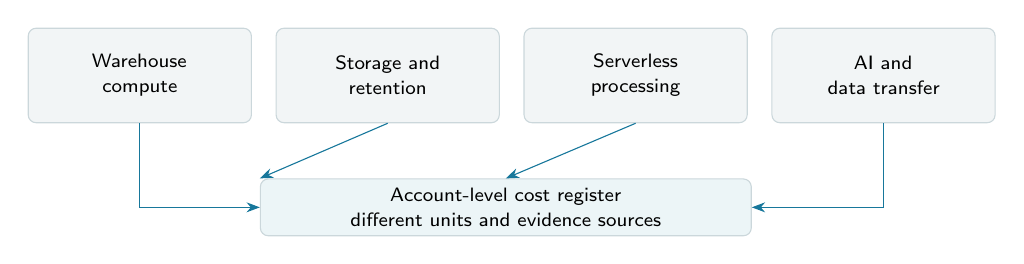
\begin{tikzpicture}[>=Stealth,every node/.style={font=\sffamily\fontsize{7.5}{9}\selectfont},n/.style={draw=thinrule,rounded corners=1mm,fill=papergray,align=center,text width=26mm,minimum height=12mm}]
\node[n](wh){Warehouse\\compute};\node[n,right=3mm of wh](st){Storage and\\retention};\node[n,right=3mm of st](sl){Serverless\\processing};\node[n,right=3mm of sl](ai){AI and\\data transfer};
\node[draw=thinrule,rounded corners=1mm,fill=lightblue,align=center,below=7mm of st,xshift=15mm,text width=60mm](bill){Account-level cost register\\different units and evidence sources};
\draw[->,steelblue](wh.south) |- (bill.west);\draw[->,steelblue](st.south) -- (bill.north west);\draw[->,steelblue](sl.south) -- (bill.north);\draw[->,steelblue](ai.south) |- (bill.east);
\end{tikzpicture}\\{\fontsize{8}{9}\selectfont\color{inkgray}Figure 13.5. A warehouse-only cost report is not a complete bill.}\end{center}
\begin{whitebox}\textbf{Cost category checklist}\par
For each charge, record a service name, usage period, resource or owner, raw quantity and unit, published or contracted price source, currency, taxes if relevant, data freshness, and whether the number is measured, modeled or illustrative. A missing cost category should be reported as unknown, not zero.
\end{whitebox}
A fixed-cost spreadsheet is suitable for checking scenario arithmetic, but not for proving the availability or price of a cloud feature. Keep version-specific rates in a reviewed external configuration file and capture the date and region of every quoted figure.
\textbf{Check.} Why might an account have modest virtual-warehouse usage yet a materially larger total cloud bill?
\newpage
% PAGE 241
\topic{13.7.3}{Unit economics and cost attribution}
Cost attribution connects a spend category to a decision maker. Shared warehouses complicate this because idle time, queued requests and queries from different teams overlap. Query attribution can estimate execution compute by query, but it does not automatically allocate all warehouse idle time, storage, cloud-service overhead, serverless services or AI usage. One honest accounting method reports warehouse metering as a source of truth, then assigns allocation rules with disclosed assumptions. Never add attributed query credits to the same warehouse's billed credits.
\begin{lstlisting}[language=SQL,caption={Separate per-query attributed compute, not an extra charge.}]
SELECT COALESCE(NULLIF(query_tag, ''), 'untagged')
         AS workload,
       SUM(credits_attributed_compute) AS query_credits
FROM SNOWFLAKE.ACCOUNT_USAGE.QUERY_ATTRIBUTION_HISTORY
WHERE start_time >= DATEADD(day, -7, CURRENT_DATE())
GROUP BY workload
ORDER BY query_credits DESC;
\end{lstlisting}
Assign workload-level \texttt{QUERY\_TAG}s during ETL, API serving and scheduled reporting; tag shared physical resources with their cost center where appropriate. Record untagged usage and the governance process for correcting it. Avoid putting secret or personal information in query tags. For a complete monthly report reconcile metering and billing on the same reporting boundary, with a documented treatment of delays and adjustments.

\begin{whitebox}\textbf{Unit economics, with denominators}\par
If an illustrative weekly run consumes 12 credited units for 24 accepted batches, cost is 0.5 credits per batch. If the same input creates 2400 accepted observations, it is 0.005 credits per observation. These values describe the modeled run only. Always state the denominator, excluded categories, data quality, and actual or assumed credit quantity before using a ratio for planning.
\end{whitebox}
Cost per dashboard load, per fresh MWh observation and per validated file measure different products. Choose metrics tied to a business service-level expectation, and reject a cost reduction that simply skips data validation or reduces refreshes below the agreed tolerance.
\repo{P151: Example Snowflake cost monitoring}{https://github.com/Matatika/example-snowflake-cost-monitoring}
\textbf{Check.} How would you fairly apportion a warehouse's idle expense across teams, and what assumptions would the resulting dashboard expose?
\newpage
% PAGE 242
\section*{13.8\quad Budgets, monitoring, and workload guardrails}
\topic{13.8.1}{Resource Monitors and their scope}
Snowflake Resource Monitors primarily govern supported warehouse credit consumption: they can notify and apply suspend actions to monitored user-managed warehouses at configured thresholds. They are not universal spending caps, cannot stop every in-flight operation immediately, and do not cover serverless or AI service consumption. Test notification recipients and stop behavior in a restricted environment rather than trusting configuration names alone.
\topic{13.8.2}{Budgets and alert response}
Budgets monitor supported consumption against a defined spending target and forecast; they issue alerts when a threshold is or may be exceeded, depending on configuration. A budget is not a general-purpose hard shutoff. Route alerts to an accountable owner with explicit escalation, and confirm whether each relevant service is included in its scope. Alert noise without a response owner is only another operational failure.
\topic{13.8.3}{Stop conditions and cost incident handling}
Define two thresholds: an early-review threshold that triggers diagnosis and an emergency stop condition authorizing suspension of particular approved workloads. Before stopping, assess safety and data freshness implications. A necessary daily compliance report should not vanish because an unrelated experimental warehouse consumed credits. Pause the experiment first; capture query history, warehouse ownership, expected next run and the recovery plan.
\begin{whitebox}\textbf{Illustrative two-stage response}\par
At 70\% of a modeled monthly allocation, the owner checks anomalous resource usage. At 90\%, the owner requests a scoped review and pauses nonessential experiments where authorized. These percentages are an organizational exercise, not Snowflake defaults or claims of fixed enforcement behavior.
\end{whitebox}
\repo{P152: AI cost governance example}{https://github.com/sfc-gh-sochandra/ai-cost-governance}
\textbf{Check.} Which charges can continue even when every monitored virtual warehouse is suspended?
\newpage
% PAGE 243
\section*{13.9\quad Operational reliability, recovery, and incident response}
\topic{13.9.1}{Recoverability, backups, and limits}
Snowflake Time Travel permits supported historical queries and restoration within the configured retention period; Fail-safe is a platform-assisted recovery mechanism rather than an ordinary customer backup or instant rollback. Edition, object type and retention settings matter. An independent export, replicated environment or protected source replay may be required for a business recovery promise. Test actual recovery from an isolated object, including grants and dependent applications; do not assume that cloned data includes every service, stage or operational integration.
\topic{13.9.2}{Runbook-driven incident response}
Define states: \emph{detect, triage, contain, recover, verify, communicate, learn}. Assign roles for incident commander, technical responder, data steward and stakeholder communications. Preserve necessary logs before cleanup, but restrict incident artifacts because they can contain identities or other sensitive details. For a mistakenly broadened role, containment may mean revoking an inheritance edge and rotating a secret, not destroying the affected table.
\topic{13.9.3}{RPO/RTO and testing recovery drills}
Recovery Point Objective (RPO) bounds acceptable data loss; Recovery Time Objective (RTO) bounds restoration time. These are negotiated business requirements, not automatic guarantees provided by any single Snowflake feature. A dry run should include detection delay, re-establishing credentials, rebuilding a scheduled task, replaying missing events, checking accepted counts and restoring dashboard freshness.
\begin{whitebox}\textbf{Recovery drill acceptance}\par
Simulate a broken gold table in a disposable sandbox. Record the incident start, suspected loss window, steps taken, actual data restored, check totals and achieved time to recovery. If the result exceeds the target, record the gap and follow-up; do not silently change the target after observing the outcome.
\end{whitebox}
\repo{P153: Snowflake failover script reference}{https://github.com/Snowflake-Labs/sfguide_failover_scripts}
\textbf{Check.} If a consumer can tolerate one hour of delayed reporting but no permanently missing confirmed reading, how would the RPO and RTO differ?
\newpage
% PAGE 244
\section*{13.10\quad Governance and platform runbooks}
\topic{13.10.1}{Governance ownership assignments}
A governance council is not needed for every small data team, but every critical data product needs named decision owners. The platform owner controls Snowflake configuration and reliability; the data owner approves legitimate uses; the steward maintains definitions and quality thresholds; the security owner authorizes controls; finance approves spending thresholds; the product owner resolves delivery trade-offs. One person may fill several roles in a small team, but conflicting approvals should receive independent review.
\begin{whitebox}\textbf{Example responsibility table}\par
\begin{tabularx}{\linewidth}{>{\raggedright\arraybackslash}X>{\raggedright\arraybackslash}X>{\raggedright\arraybackslash}X}
\toprule
Decision & Accountable & Required evidence \\
\midrule
Share a new KPI & Data owner & Contract and recipient scope \\
Change masking & Security owner & Policy test and review \\
Change warehouse size & Platform owner & Cost/latency benchmark \\
Delete a source history & Data/privacy owner & Retention and recovery review \\
\bottomrule
\end{tabularx}
\end{whitebox}
\textbf{Avoid governance theater.} Naming roles in a slide is not control. Add a reliable queue for requests, explicit response time, delegation rules, documented approval evidence and a mechanism for correcting mistakes. Ensure platform teams can answer simple questions promptly: who owns this table, what is the data classification, who may read it, when did it last refresh, and who pays for it?
\begin{lstlisting}[language=SQL,caption={A neutral context probe for a governed change request.}]
SELECT CURRENT_ACCOUNT(), CURRENT_ROLE(),
       CURRENT_DATABASE(), CURRENT_SCHEMA();
-- Never attach personal identifiers or credentials to
-- the query tag or shared approval ticket.
\end{lstlisting}
\repo{P154: SnowAlert policy monitoring reference}{https://github.com/snowflakedb/SnowAlert}
\textbf{Check.} If a sensitive field moves into a newly published view, whose approval is required and what artifact proves it occurred?
\newpage
% PAGE 245
\topic{13.10.2}{Audit evidence and recurring reviews}
Operational evidence degrades unless reviewed. A monthly security review compares effective role grants to the approved matrix, identifies dormant service identities and checks high-risk policy changes. A weekly data quality review checks freshness, rejected records, duplicate rate, accepted volume and incident backlog. A cost review reconciles billed categories to owners and follows up untagged workloads. Quarterly, run a recovery drill and reassess retention and sharing inventory.

Record failures as well as passes. A security test skipped because an Enterprise-only feature was unavailable is not equivalent to a successful test. Mark it \textbf{not executed} and identify the control that substitutes in the lab, such as a restricted secure view or a separate account-level verification path. Similarly, an offline cost register validates arithmetic but cannot establish billed Snowflake credits or quoted EUR figures.
\begin{whitebox}\textbf{Evidence bundle for release \texttt{13.0-lab}}\par
\texttt{security\_policies.sql}: proposed policy DDL with privileges and review gates.\par
\texttt{security\_tests.sql}: expected permitted and denied SQL, to run under real authorized users.\par
\texttt{cost\_register.csv}: synthetic usage assumptions and unit labels.\par
\texttt{incident\_runbook.md}: stepwise containment and recovery.\par
\texttt{tests/}: executed offline test output and limitations.\par
\texttt{QUALITY\_REPORT.txt}: scope, test status, result summary and required cloud checks.
\end{whitebox}
A review should ask about \emph{control drift}: did a legitimate shortcut create a long-lived privilege, did an analytics-only service gain insert access, or did a new AI workload bypass the ownership budget? Drift can arise even when every single earlier change was approved, because the combined state of the system changed.

\textbf{Decision point.} Prefer the least invasive remediation consistent with safety: remove an accidental role edge before restructuring an entire database, lower experimental schedule frequency before disabling every report, or fix a model contract before creating a new layer of data copies.
\textbf{Check.} Which required evidence distinguishes a policy that was proposed in Git from a policy actually deployed and verified under the intended role?
\newpage
% PAGE 246
\topic{13.10.3}{Platform operating procedures and checklists}
A runbook must work when the engineer who wrote it is asleep. Use imperative steps, with preconditions, approval scope and rollback. Include how to detect the trigger, confirm account and role, preserve evidence, contain safely, verify the data contract, communicate impact, and retire temporary privileges. Keep commands explicit about whether they are read-only, privileged or destructive. If a user cannot tell whether \texttt{DROP} deletes lab-only resources, it does not belong in a copy-and-run recovery procedure.
\begin{whitebox}\textbf{One-page operational checklist}\par
\begin{enumerate}
\item Identify incident ID, severity, time window, affected data product and owner.
\item Verify account, region, role, active secondary roles and required approvals.
\item Preserve query IDs, grant snapshots, scheduled-job status and cost context.
\item Apply the smallest authorized containment action; log its exact effects.
\item Recover from tested source replay, retained history or approved backup.
\item Reconcile row counts, units, watermark, 66.000 MWh fixture invariant, and freshness.
\item Rerun permitted and denied access tests; restore alert routing and schedules.
\item Notify consumers, record follow-ups, remove temporary rights, schedule review.
\end{enumerate}
\end{whitebox}
\textbf{Example: runaway experimental load.} An alert identifies the book lab warehouse as unexpectedly active. Confirm no critical work shares it; capture active statement IDs; notify the owner; suspend the isolated warehouse if authorized; inspect query history and schedule; record total actual metered credits when data becomes available; restart only after fixing the cause. Do not claim the monitor can stop all future serverless or AI activity.

\textbf{Example: unauthorized raw access.} Confirm effective role and identity, revoke the unintended grant edge, rotate any exposed credential, assess data exposure and preserve evidence. Do not hide the incident by truncating tables or deleting audit records. A follow-up change must include positive and negative access assertions from approved test users and an explicit review of inherited permissions.
\repo{P155: Application control framework}{https://github.com/Snowflake-Labs/sfguide-application-control-framework}
\textbf{Check.} Could an on-call engineer locate the right owner, determine whether to stop a pipeline, and prove it is safe to resume?
\newpage
% PAGE 247
\section*{13.L\quad Guided lab, chapter review, and exercises}
\topic{13.L.1}{Prerequisites, inputs, environment, permissions, and cost guardrails}
The companion \texttt{lab/} directory contains an original author-written security and cost exercise, not copied repository code. Its source fixture is synthetic: six accepted energy observations total 66.000 MWh. The optional cloud steps use disposable \texttt{BOOK13\_SANDBOX} objects. Obtain explicit approval for role creation, grants and masking policy application; enterprise-only features may not be available. Avoid \texttt{ACCOUNTADMIN} for notebook execution and never embed real secrets.
\begin{whitebox}\textbf{Preflight decisions}\par
\textbf{Execution profile A (default):} local Python tests; no Snowflake credentials, no cloud billing, no personal data.\par
\textbf{Profile B (optional):} approved disposable Snowflake account; restricted provisioning identity, dedicated small auto-suspending warehouse, documented credit guardrail and verified cleanup plan. Run security negative cases with two separate approved identities; never assume inherited rights away.
\end{whitebox}
\topic{13.L.2}{Step-by-step procedure with selected code and illustrative results}
\begin{enumerate}
\item Review \texttt{security\_policies.sql} and approve object and role names. Run read-only inventory first.
\item In a disposable environment, provision the synthetic \texttt{GOLD.GENERATION\_DAILY} object and narrow reader access. Apply masking only where supported, approved and independently reviewed.
\item Run \texttt{security\_tests.sql} under each designated identity and verify the explicit allow/deny matrix. Record query IDs and denial causes.
\item Run local \texttt{python -m unittest discover -s tests -v} to validate the offline access graph, cost ledger, and runbook invariant checks.
\item Fill \texttt{cost\_register.csv} with scenario consumption; keep actual Snowflake metering and monetary rate separate until verified.
\item Rehearse access and cost incidents using the companion runbook. Record detection, containment, verification and handoff times.
\end{enumerate}
\begin{lstlisting}[language=SQL,caption={Illustrative approved-reader test in an isolated account.}]
SELECT CURRENT_USER(), CURRENT_ROLE();
SELECT COUNT(*) AS rows_visible
FROM BOOK13_SANDBOX.GOLD.GENERATION_DAILY;
-- Separate unauthorized test: expected denied.
SELECT COUNT(*) FROM BOOK13_SANDBOX.RAW.METER_EVENT;
\end{lstlisting}
Expected result of the offline fixture: six accepted observations, total 66.000 MWh; no asserted cloud result. Account behavior, denial text, edition constraints and metered credits must be recorded after a real supervised run.
\newpage
% PAGE 248
\topic{13.L.3}{Expected result, assertions, failure diagnosis, rollback, and cleanup}
The lab passes only if approved access succeeds, forbidden actions genuinely fail with authorization errors, sensitive values are masked for unauthorized readers (if the masking feature is enabled), and the cost register reconciles assumptions without confusing estimated and observed usage. A \texttt{SQL compilation error} is not proof of least privilege. The offline suite verifies scenario rules and metadata completeness; its passing status does not establish Snowflake security compliance.

If an access case unexpectedly succeeds, stop and inspect secondary roles, user grants and inherited role paths. If a masking policy is unavailable, log \emph{feature not tested} and never represent a view-based substitution as equivalent. If a bill estimate differs, verify units, minimum billing intervals and excluded services before blaming the data. Cleanup must be owner-approved, scoped to \texttt{BOOK13\_SANDBOX}, and executed from the safe checklist; destructive SQL is commented out by default.
\topic{13.L.4}{Foundation, practitioner and production design challenges}
\textbf{Concept review.} (1) Why is \texttt{SELECT} authorization different from masking? (2) How can role inheritance expand access unexpectedly? (3) What does a warehouse Resource Monitor not cover? (4) Why is Fail-safe not a general backup strategy? (5) How can a query-cost report double-count expenditure?

\textbf{Foundation exercise.} Draw a three-role access graph and write a permitted/denied action matrix. \emph{Acceptance:} no loader privilege reaches the BI reader, and every high-risk action names an owner.

\textbf{Practitioner exercise.} Extend the cost ledger to include a modeled serverless usage line and verify that the warehouse subtotal is not presented as the total account bill. \emph{Acceptance:} units, provenance, pricing assumptions and omissions are explicit.

\textbf{Architecture decision.} A partner requests regional generation data, the dashboard must recover in two hours after failure, and finance demands an auditable monthly cost ceiling. Propose sharing controls, retention policy, RPO/RTO, owner responsibilities and an alert/response route. \emph{Acceptance:} identify which controls alert, which can suspend, and which do not provide hard guarantees.
\begin{whitebox}\textbf{Scoring rubric (20 points)}\par
Correct access and test identities (5); masking/classification and sharing logic (4); separate metering categories and limits (4); runnable incident and recovery verification (4); citations, provenance and honest untested labels (3). A passing score needs at least 16 points and no critical security or fabricated-evidence claim.
\end{whitebox}
\textbf{Chapter synthesis.} Governance is what keeps a data product understandable when people, systems and threats change. Least privilege is enforceable only when denied behavior is tested; cost is controllable only when its categories are visible; recovery is believable only when rehearsed. Chapter~14 adds AI workloads to this governed platform, increasing the need for all three disciplines.
{\fontsize{7.8}{9.3}\selectfont\textbf{Authoritative references (verify before print).}\quad
\href{https://docs.snowflake.com/en/user-guide/security-access-control-overview}{[1] Access control};
\href{https://docs.snowflake.com/en/user-guide/security-column-ddm-intro}{[2] Dynamic masking};
\href{https://docs.snowflake.com/en/user-guide/security-row-intro}{[3] Row access};
\href{https://docs.snowflake.com/en/user-guide/resource-monitors}{[4] Resource monitors};
\href{https://docs.snowflake.com/en/user-guide/cost-attributing}{[5] Cost attribution};
\href{https://docs.snowflake.com/en/user-guide/data-time-travel}{[6] Time Travel};
\href{https://commission.europa.eu/law/law-topic/data-protection_en}{[7] EU data protection}.\par
\textit{Documentation checked 22 October 2026; all third-party GitHub references are leads, not independently executed or cleared for republication.}}
\end{document}
